

\documentclass[11pt]{article}
\usepackage{graphicx}
\usepackage[margin=1.25in]{geometry}
\usepackage[usenames,dvipsnames]{color}
\usepackage{url}
\usepackage[colorlinks = true,
            linkcolor = blue,
            urlcolor  = blue,
            citecolor = blue,
            anchorcolor = blue]{hyperref}
%can change bib here...
\usepackage[square,comma,sort&compress,numbers]{natbib}
\usepackage{caption}
\usepackage{subcaption}
\bibliographystyle{unsrtnat}


%%%%%%%%%%%%%%%%%%%%%%%%%%%%%%%%%%%%%%%%%%%%%%%%%%%%%%%%%%%%%%%%%%%%
% basic data for the eprint:
%%%%%%%%%%%%%%%%%%%%%%%%%%%%%%%%%%%%%%%%%%%%%%%%%%%%%%%%%%%%%%%%%%%%

\textwidth=6.0in  \textheight=8.5in

%%  Adjust these for your printer:
\parskip=0.1truein 
  
%% preprint number data:
\newcommand\pubnumber{Preprint Number Goes Here?}
\newcommand\pubdate{\today}



%%%%%%%%%%%%%%%%%%%%%%%%%%%%%%%%%%%%%%%%%%%%%%%%%%%%%%%%%%%%%%%%%%%%%%%%%%%%
%   document style macros
%%%%%%%%%%%%%%%%%%%%%%%%%%%%%%%%%%%%%%%%%%%%%%%%%%%%%%%%%%%%%%%%%%%%%%%%%%%%
\def\Title#1{\begin{center} {\LARGE #1 } \end{center}}
\def\Author#1{\begin{center}{ \sc #1} \end{center}}
\def\Address#1{\begin{center}{ \it #1} \end{center}}
\def\andauth{\begin{center}{and} \end{center}}
\def\submit#1{\begin{center}Submitted to {\sl #1} \end{center}}
\newcommand\pubblock{\rightline{\begin{tabular}{l} \pubnumber\\
         \pubdate \end{tabular}}}
\newenvironment{Abstract}{\begin{quotation} \begin{center}
                       ABSTRACT
     \end{center}\bigskip  }{\end{quotation}}
\newenvironment{Presented}{\begin{quotation} \begin{center} 
             CONTRIBUTED TO\end{center}\bigskip 
      \begin{center}\begin{large}}{\end{large}\end{center} \end{quotation}}
\def\submit#1{\begin{center}Submitted to {\sl #1} \end{center}}
\def\Acknowledgements{\bigskip  \bigskip \begin{center} \begin{large}
             \bf ACKNOWLEDGEMENTS \end{large}\end{center}}
%%%%%%%%%%%%%%%%%%%%%%%%%%%%%%%%%%%%%%%%%%%%%%%%%%%%%%%%%%%%%%%%%%%%%%%%%%%%
%  personal abbreviations and macros

\input workshopsymbols.tex

\newcommand\snowmass{\begin{center}\rule[-0.2in]{\hsize}{0.01in}\\\rule{\hsize}{0.01in}\\
\vskip 0.1in Submitted to the  Proceedings of the US Community Study\\ 
on the Future of Particle Physics (Snowmass 2021)\\ 
\rule{\hsize}{0.01in}\\\rule[+0.2in]{\hsize}{0.01in} \end{center}}

%%%%%%%%%%%%%%%%%%%%%%%%%%%%%%%%%%%%%%%%%%%%%%%%%%%%%%%%%%%%%%%%%%%%%%%%%%%
\usepackage{authblk}

\title{Summarizing experimental sensitivities of collider experiments to Dark Matter models and comparison to other experiments}

\author[1]{Antonio Boveia}
\affil[1]{The Ohio State University}
\author[2,3]{Caterina Doglioni}
\affil[2]{University of Manchester}
\affil[3]{Lund University}
\author[4]{Boyu Gao}
\affil[4]{Duke University}
\author[3]{Josh Greaves}
\author[5]{Philip Harris}
\affil[5]{MIT}
\author[6]{Katherine Pachal}
\affil[6]{TRIUMF}

% Adding contributors who gave us things directly
\author[6]{Robert Harris}
\affil[6]{Fermi National Accelerator Laboratory}
\author[7]{Tetiana Hrynova}
\affil[7]{LAPP Annecy}
\author[7]{Jared Little}
% Didn't ask Giuliano if he wants in, but he did extra work for us so it seems good to me
\author[8]{Giuliano Gustavino}
\affil[8]{CERN}

\begin{document}

%KP: the author format here is mega long, i don't love it.
% going to a more normal formatting unless someone else wants to figure out how to make this pretty
% note from Michael in this repo says this isn't obligatory anyway

% \pubblock
%\Title{Summarizing experimental sensitivities of collider experiments to Dark Matter models and comparison to other experiments}

%\bigskip 

% Adding us
\maketitle

%LOI authors:
%\noindent{\large \bf Authors: }Antonio Boveia (Ohio State University), Linda Carpenter (Ohio State University), Caterina Doglioni (Lund University), William Kalderon (Brookhaven National Lab), Boyu Gao (Ohio State University), Philip Coleman Harris (Massachusetts Institute of Technology), David Yu (Brown University)\\

%\medskip

%\Address{ c/o  R. W. Emerson, Concord, MA USA}

\medskip

 \begin{Abstract}
\noindent Plots summarizing the constraints on Dark Matter (DM) models can help visualize synergies between different searches for the same kind of experiment, as well as between different experiments. 
In this LOI, we propose to produce these plots from the perspective of collider searches within EF10 starting from inputs from future collider facilities. We will take as a starting point the plots currently made for LHC searches and recommended by the Dark Matter Working Group, also used for the BSM and Dark Matter chapters of the European Strategy Briefing Book. We also intend to actively participate in the cross-frontier discussions about dark matter complementarity. This is a whitepaper submitted to the APS Snowmass process for the EF10 topical group. 
\end{Abstract}


\snowmass

\def\thefootnote{\fnsymbol{footnote}}
\setcounter{footnote}{0}
%

\section{Introduction}

Collider experiments searching for dark matter can constrain a wide variety of models of dark matter production in hadron or lepton collisions. Underground and above-ground direct-detection experiments can constrain the interaction rate of dark matter in our solar neighborhood with nuclei and electrons, and [indirect-detection/telescopes] can constrain self-annihilation of dark matter beyond our local neighborhood. Nevertheless, putting together the information learned from these different types of particle physics experiments is challenging, since it requires a model, and we have few clues as to what the correct model of  dark matter might be.

One model framework long used to connect dark matter searches is supersymmetry. [But this is not really the correct tool for the job: it does a lot more than describe DM; has many parameters, many of which have nothing to do with DM; and need not provide a DM candidate at all]. Recently, some DM experiments, primarily at the LHC [but not restricted to it] use simplified models for this purpose. Fewer parameters, allow focus on low-energy phenomenology at the experiments, at the expense of theoretical completeness and unambiguous connection to the observed galactic abundance of DM. With fewer parameters, easier to construct slices of parameter space to make rough/quantitative-but-fragile comparisons of experimental coverage.

In this whitepaper, we use the [comparisons within simplified models approach] to visualize projected sensitivities of future collider experiments to DM production and their relationship to the projected sensitivities of proposed direct detection and indirect detection searches. These projections have been prepared within the EF10 topical group starting from a selection of projections provided by studies of future collider facilities. The simplified models used consist of those recommended by the LHC Dark Matter Working Group and currently used by LHC searches, as well as in the BSM and Dark Matter chapters of the recent European Strategy Briefing Book. 

\section{Future collider facilities}
\label{sec:colliders}

Summarise the inputs we received and what their parameters are

So far: HL-LHC, FCC-hh. 
List of inputs received and relevant citations:
\begin{itemize}
    \item HL-LHC monojet~\cite{hllhc-monojet}
    \item HL-LHC and FCC dijet~\cite{Harris:2022kls}
    \item FCC monojet [cite Phil]
    \item HL-LHC dilepton, ATLAS [cite Tanya and Jared]
    \item HL-LHC diilepton, CMS [cite that PAS, but limits not actually in the plots yet]
\end{itemize}

\section{Plots summarizing collider reach to dark matter mediator models}

\subsection{Previous text from LOI}

To compare how existing collider searches may discover or constrain a given model, and to understand how future collider experiments would extend these results, we propose to make summary plots like Figure\ref{fig:Fig1} ~\cite{CMSSummary,ATL-PHYS-DMSUM-JHEP-2019} in terms of the fundamental parameters of the Lagrangian of a model. 
Exclusion comparisons in the DM mass – mediator mass plane (left panel) combine searches for both invisible and visible signals of the model. Summary plots such as on the mediator – quark coupling and mediator mass plane (right panel) target the production coupling and visible decay of the mediator. For both types of plots, we suggest using DM simplified models~\cite{ABERCROMBIE2020100371} since they are simple descriptions of collider phenomenology that capture common features across many full models, while ignoring the differences among these models at energies higher than collider scales~\cite{doi:10.1146/annurev-nucl-101917-021008}. In the simplified models, the interaction between Standard Model (SM) particles and DM is mediated by a new particle called a mediator, where the mediator – quark coupling controls the interaction strength between mediator and SM quarks. These models can also be used as a stepping stone to connect collider searches to accelerator searches since these results can be reinterpreted using different portal models~\cite{Beacham:2652223}, as the simplified models we are using are very close to other portal models. 

% KP removing old figures.
%\begin{figure}[ht]
%\begin{tabular}{ll}
%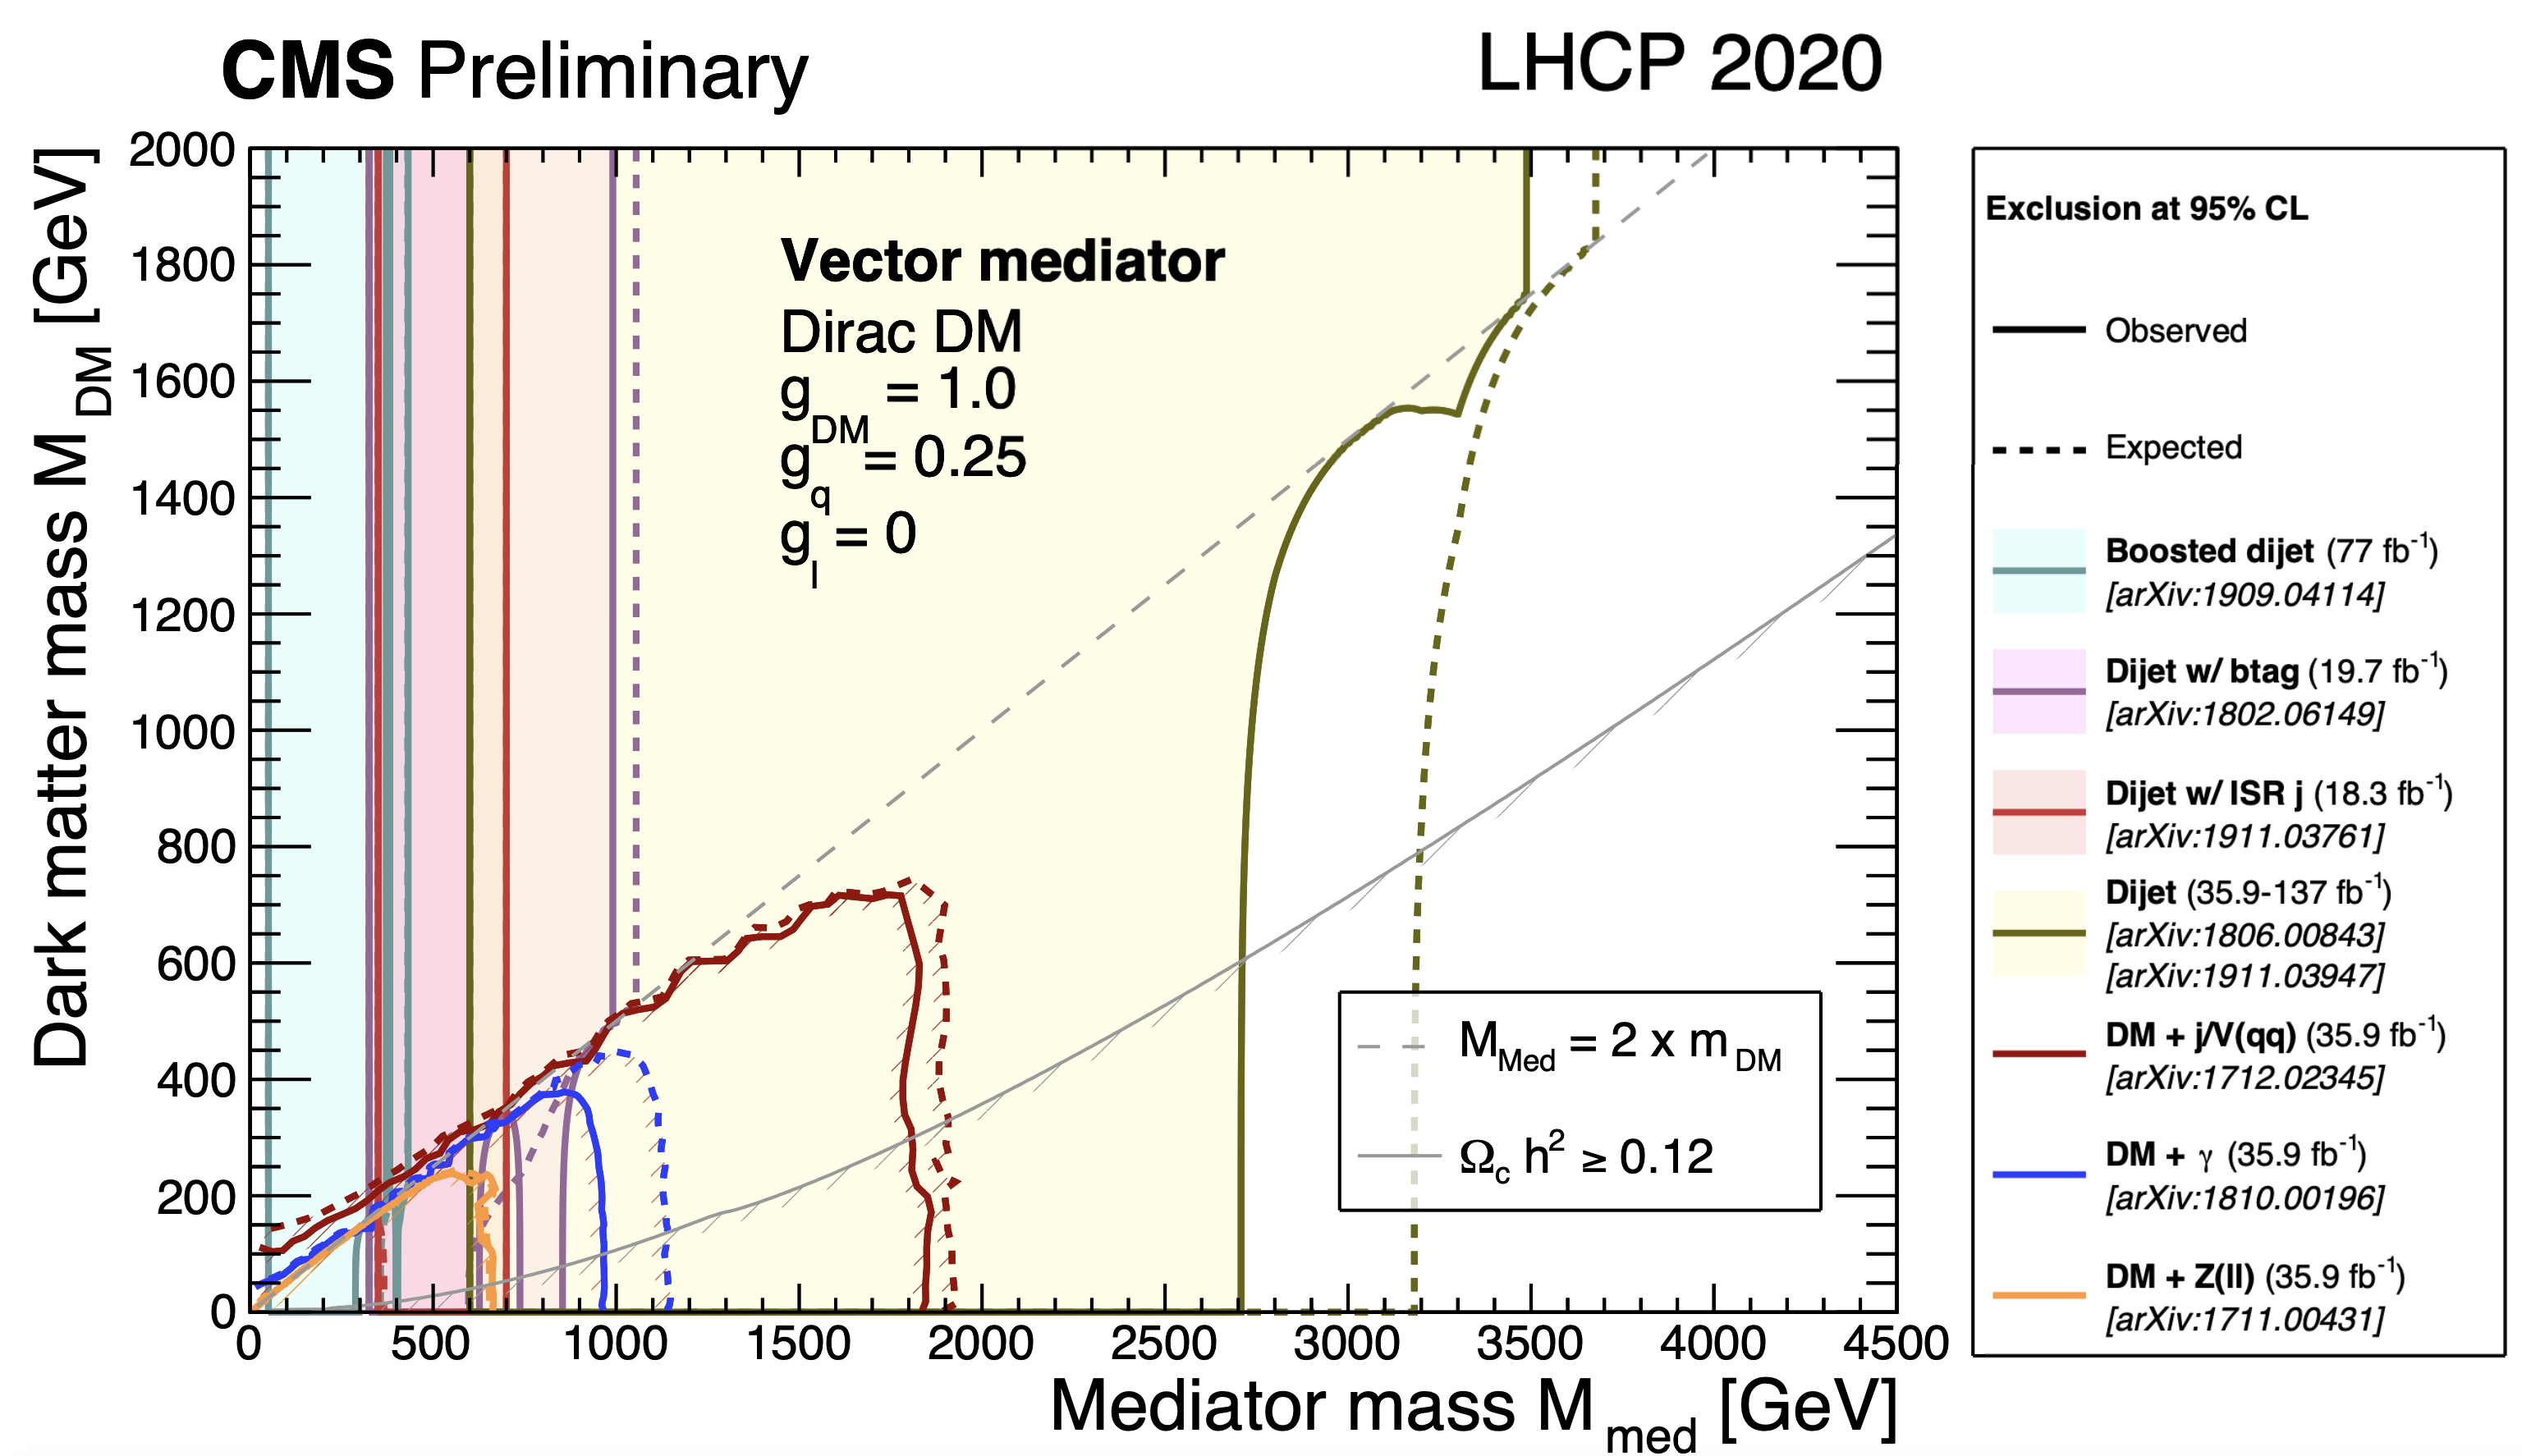
\includegraphics[scale=0.17]{figures/DMsummaryplots_med_dm.png}
%&
%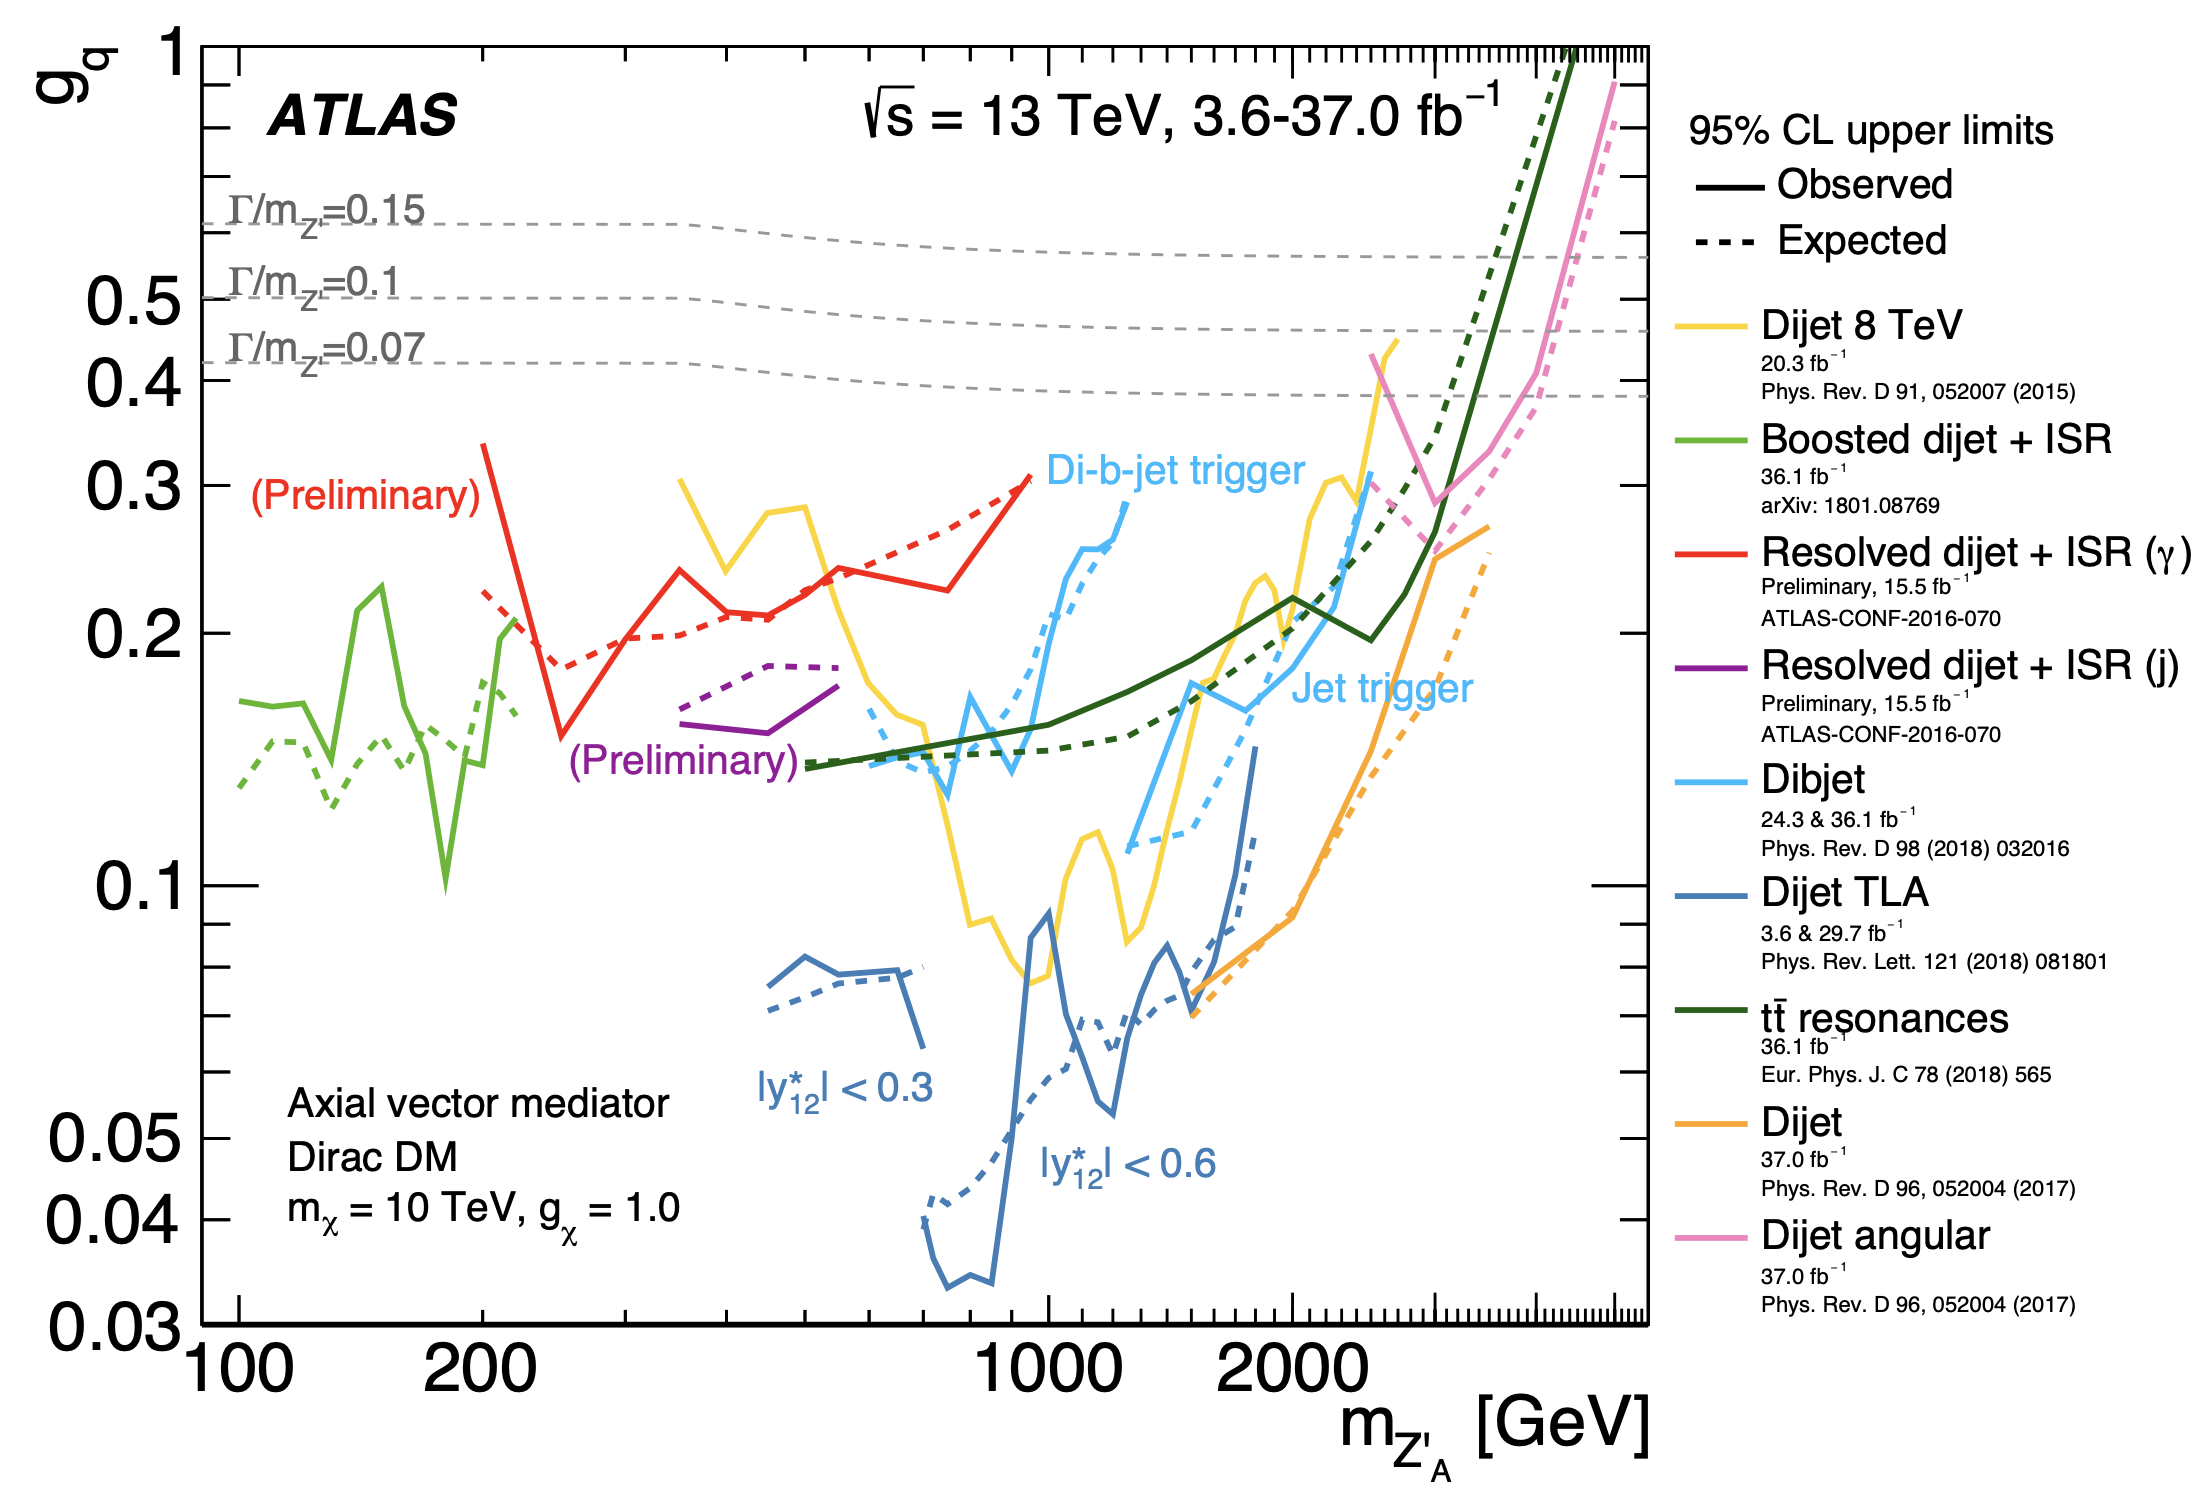
\includegraphics[scale=0.185]{figures/DMsummaryplots_med_gq.png}
%\end{tabular}
%\caption{{\bf Left panel}: regions in DM mass - mediator mass plane excluded at 95$\%$ CL by visible and invisible searches for DM vector simplified models. {\bf Right panel}: Dijet search contours for 95$\%$ CL upper limits on the coupling $g_{q}$ as a function of resonance mass $m_{Z'_{A}}$ for axial-vector simplified models. The expected limits from each search are indicated by dotted lines. Left panel adapted from CMS Dark Matter summary plots~\cite{CMSSummary}, right panel adapted from ATLAS Dark Matter summary plots~\cite{ATL-PHYS-DMSUM-JHEP-2019}.
%}
%\label{fig:Fig1}
%\end{figure}

\subsection{Models considered}

Only vector and axial vector.

\subsection{Results}

The exclusion limits for HL-LHC and FCC-hh are interpreted in the vector and axial-vector models and scaled to a representative set of coupling values. For HL-LHC, all three of monojet, dijet, and dilepton expected limits were available. For FCC-hh, only monojet and dijet limits were available. Therefore, the set of couplings explored in the HL-LHC scenario involved varying both $g_q$ and $g_l$ while for FCC-hh only scans of $g_q$ are given here since the impact of varying $g_l$ is not significant for the monojet and dijet final states.

Figure~\ref{fig:hl-lhc-massmass-separate} shows the three projected analysis limits for HL-LHC in the vector model for a representative selection of coupling points, including the traditional ``V1'' and ``V2'' alongside alternatives.  Note the lack of dilepton line appearing in~\ref{subfig:vector-hl-lhc-v2}: \ldots [probably due to lower end of mass range being so high - go check]

\begin{figure}
     \centering
     \begin{subfigure}[b]{0.49\textwidth}
         \centering
         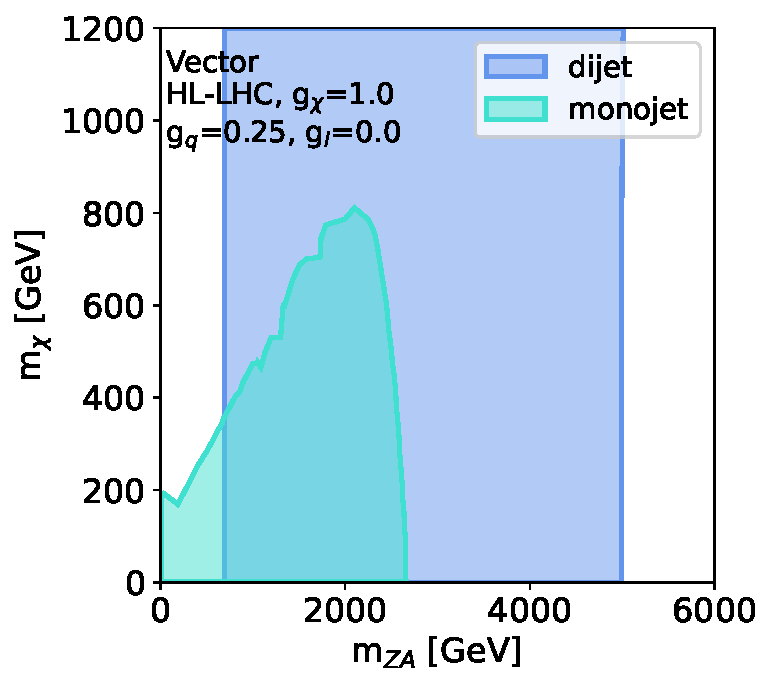
\includegraphics[width=\textwidth]{SummaryPlots-EF10/figures/massmass/hl-lhc/massmass_vector_gq0.25_gdm1.0_gl0.0.pdf}
         \caption{``V1'': $g_q=0.25$, $g_{\chi}=1.0$, $g_l=0.0$}
         \label{subfig:vector-hl-lhc-v1}
     \end{subfigure}
     \hfill
     \begin{subfigure}[b]{0.49\textwidth}
         \centering
         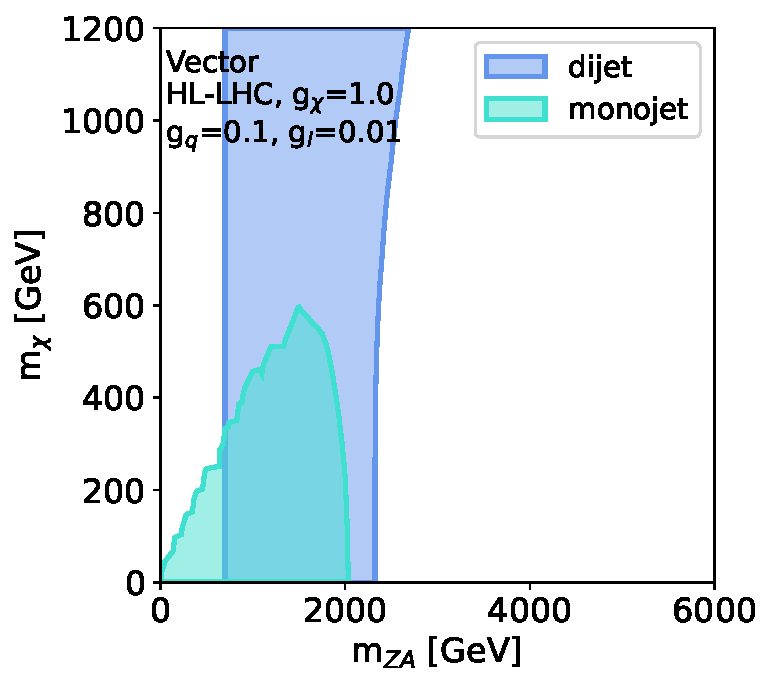
\includegraphics[width=\textwidth]{SummaryPlots-EF10/figures/massmass/hl-lhc/massmass_vector_gq0.1_gdm1.0_gl0.01.pdf}
         \caption{``V2'': $g_q=0.1$, $g_{\chi}=1.0$, $g_l=0.01$}
         \label{subfig:vector-hl-lhc-v2}
     \end{subfigure}

     \begin{subfigure}[b]{0.49\textwidth}
         \centering
         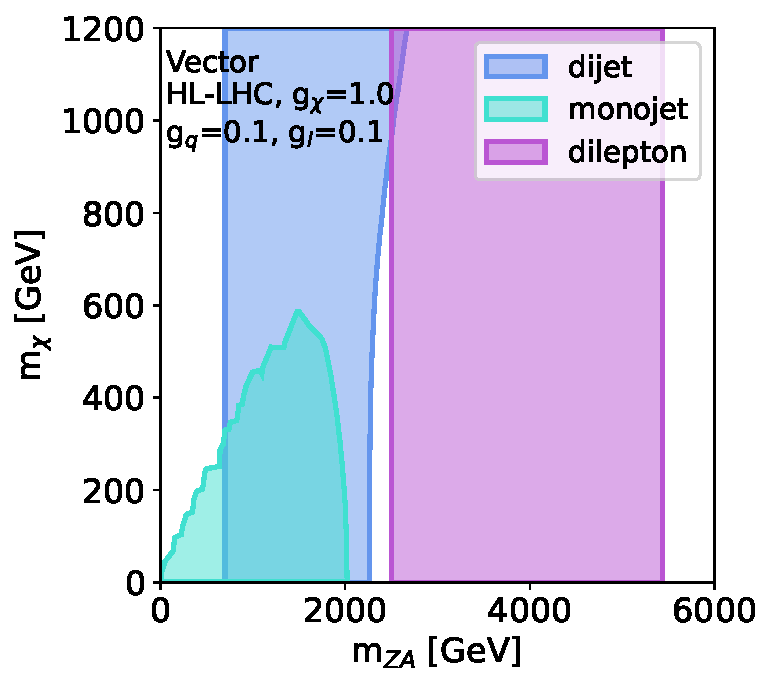
\includegraphics[width=\textwidth]{SummaryPlots-EF10/figures/massmass/hl-lhc/massmass_vector_gq0.1_gdm1.0_gl0.1.pdf}
         \caption{New scenario with varied SM couplings: $g_q=0.1$, $g_{\chi}=1.0$, $g_l=0.1$}
         \label{subfig:vector-hl-lhc-biggerlepton}
     \end{subfigure}
     \hfill
     \begin{subfigure}[b]{0.49\textwidth}
         \centering
         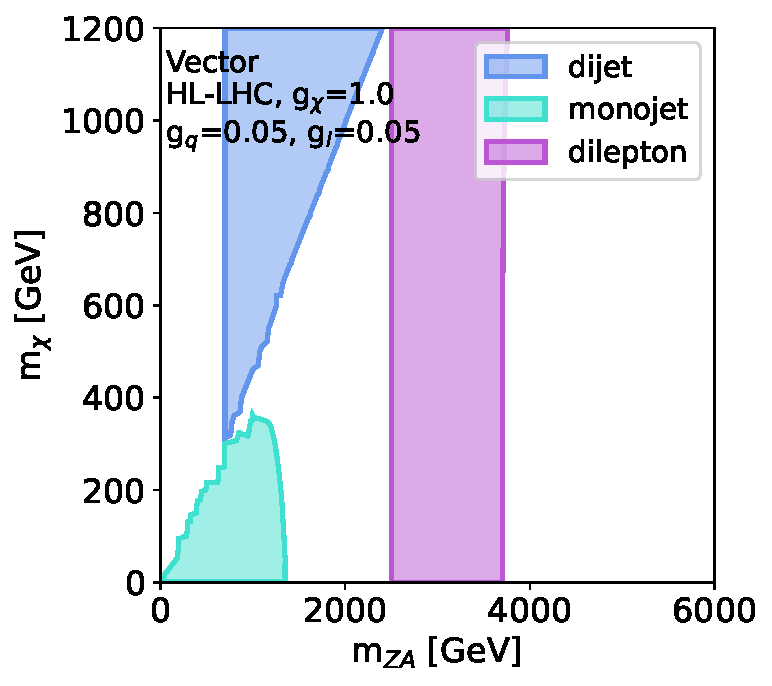
\includegraphics[width=\textwidth]{SummaryPlots-EF10/figures/massmass/hl-lhc/massmass_vector_gq0.05_gdm1.0_gl0.05.pdf}
         \caption{New scenario with varied SM couplings: $g_q=0.05$, $g_{\chi}=1.0$, $g_l=0.05$}
         \label{subfig:vector-hl-lhc-allsmall}       
     \end{subfigure}
        \caption{HL-LHC projected limits for individual analyses in the vector model and with a range of couplings.}
        \label{fig:hl-lhc-massmass-separate}
\end{figure}

In Figure~\ref{fig:hl-lhc-massmass-combined}, curves of different shades illustrate the effect on the overall excluded region of varying the couplings. A single contour is shown for each set of couplings, corresponding to the total excluded region from all three input HL-LHC analyses. With the other two couplings held constant, the remaining coupling is varied and the effects on the exclusion region shown. For simplicity, only the standard model couplings are varied, while $g_{\chi}$ is held at 1.0 in all cases. 

\begin{figure}
     \centering
     \begin{subfigure}[b]{0.49\textwidth}
         \centering
         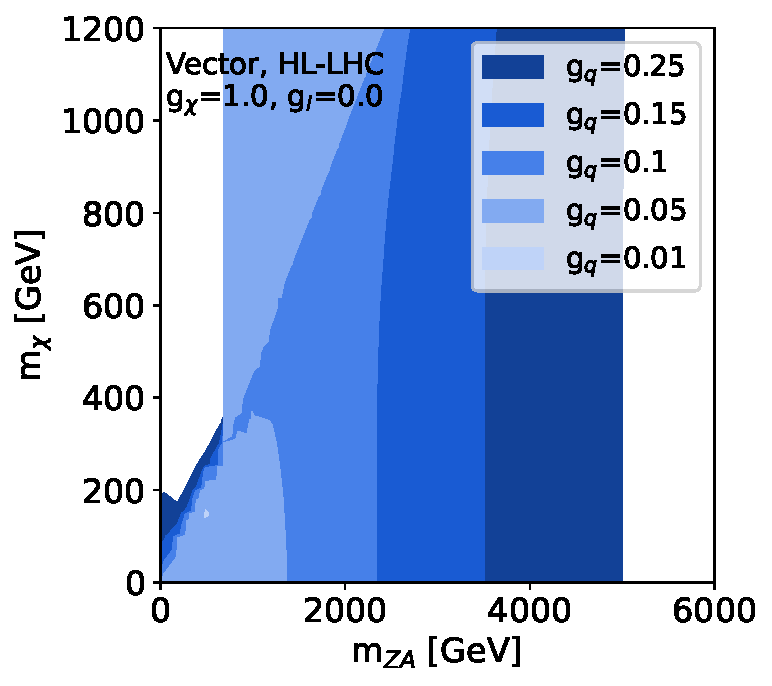
\includegraphics[width=\textwidth]{SummaryPlots-EF10/figures/massmass/hl-lhc/massmass_vector_gl0.0_gdm1.0.pdf}
         \caption{Effects of varying $g_q$ coupling with no coupling to leptons}
         \label{subfig:vector-hl-lhc-gqvariations1}
     \end{subfigure}
     \hfill
     \begin{subfigure}[b]{0.49\textwidth}
         \centering
         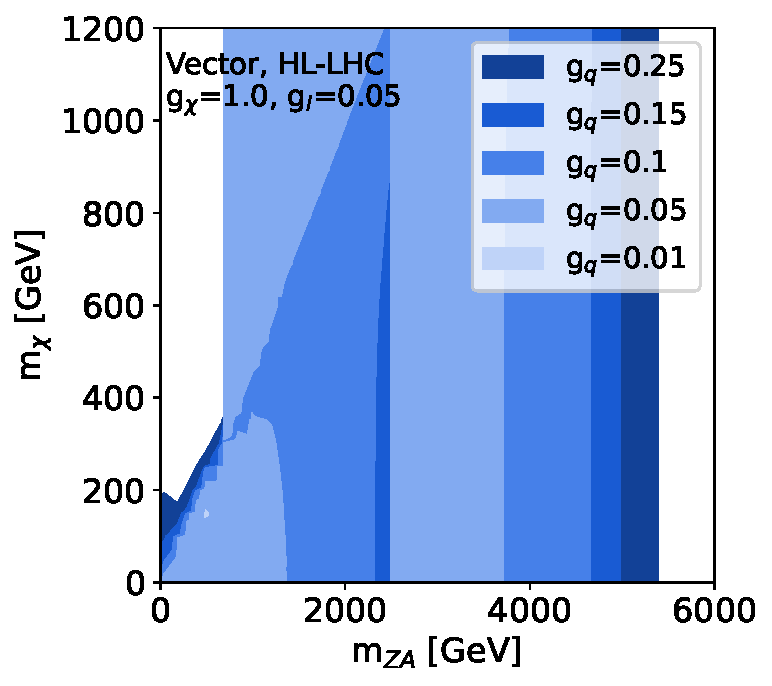
\includegraphics[width=\textwidth]{SummaryPlots-EF10/figures/massmass/hl-lhc/massmass_vector_gl0.05_gdm1.0.pdf}
         \caption{Effects of varying $g_q$ coupling with $g_l$ fixed to 0.05}
         \label{subfig:vector-hl-lhc-gqvariations2}
     \end{subfigure}

     \begin{subfigure}[b]{0.49\textwidth}
         \centering
         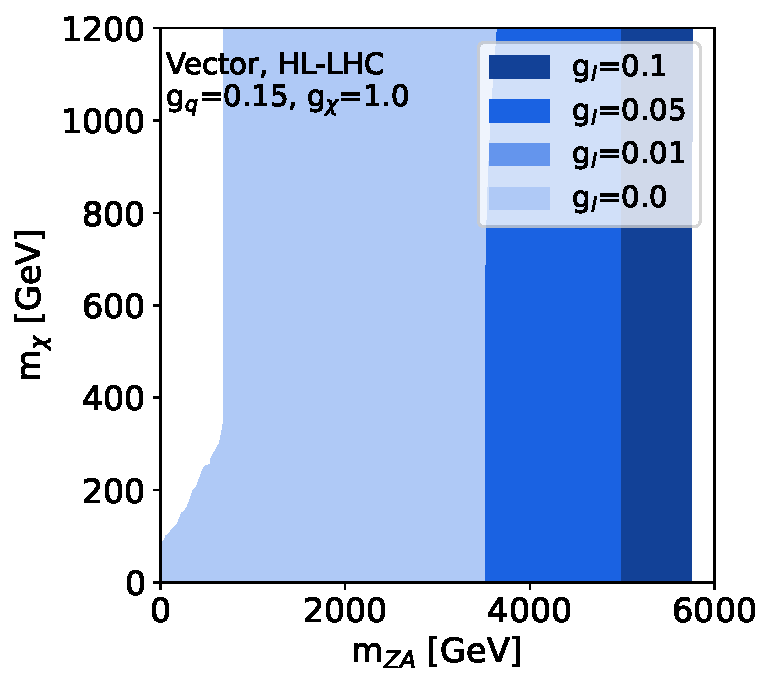
\includegraphics[width=\textwidth]{SummaryPlots-EF10/figures/massmass/hl-lhc/massmass_vector_gq0.15_gdm1.0.pdf}
         \caption{Effects of varying $g_l$ coupling with $g_q$ fixed to 0.15}
         \label{subfig:vector-hl-lhc-glvariations1}
     \end{subfigure}
     \hfill
     \begin{subfigure}[b]{0.49\textwidth}
         \centering
         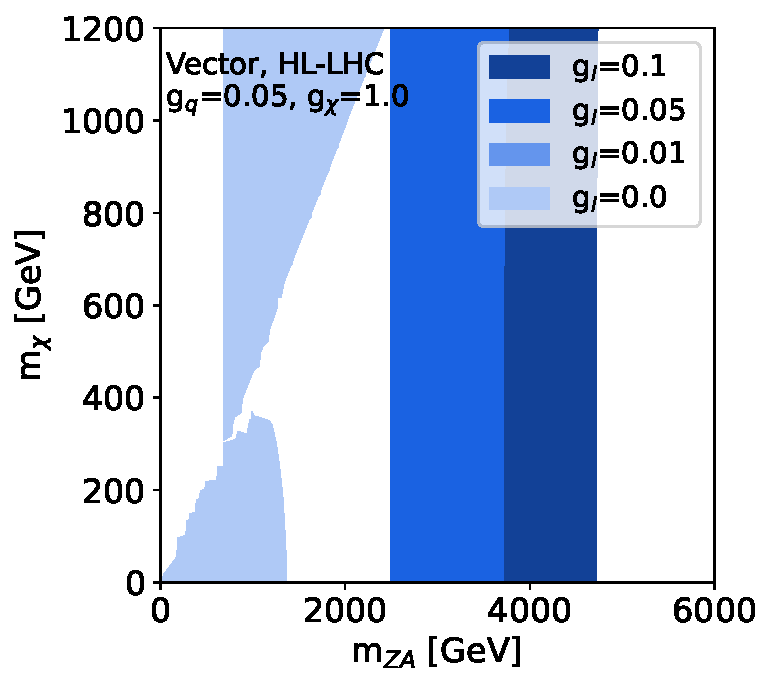
\includegraphics[width=\textwidth]{SummaryPlots-EF10/figures/massmass/hl-lhc/massmass_vector_gq0.05_gdm1.0.pdf}
         \caption{Effects of varying $g_l$ coupling with $g_q$ fixed to 0.05}
         \label{subfig:vector-hl-lhc-glvariations2}       
     \end{subfigure}
        \caption{HL-LHC projected limits, combined across analyses, for varying coupling values.}
        \label{fig:hl-lhc-massmass-combined}
\end{figure}

For FCC-hh, only dijet and monojet projections are currently available. Figure~\ref{fig:fcc-hh-massmass-separate} shows these two analysis limits for 100 TeV CME at [don't recall luminosity] in the vector model for a selection of interesting coupling points. In the absence of a dilepton prediction, the limits show little change with $g_{l}$, so the selected points vary $g_q$ only. Note that the highlighted $g_q$ values are significantly smaller than for the HL-LHC projections: this reflects the significantly greater exclusion power of FCC-hh, such that the familiar scenarios $g_q = 0.25$ are too strongly excluded to be of much interest.

\begin{figure}
     \centering
     \begin{subfigure}[b]{0.49\textwidth}
         \centering
         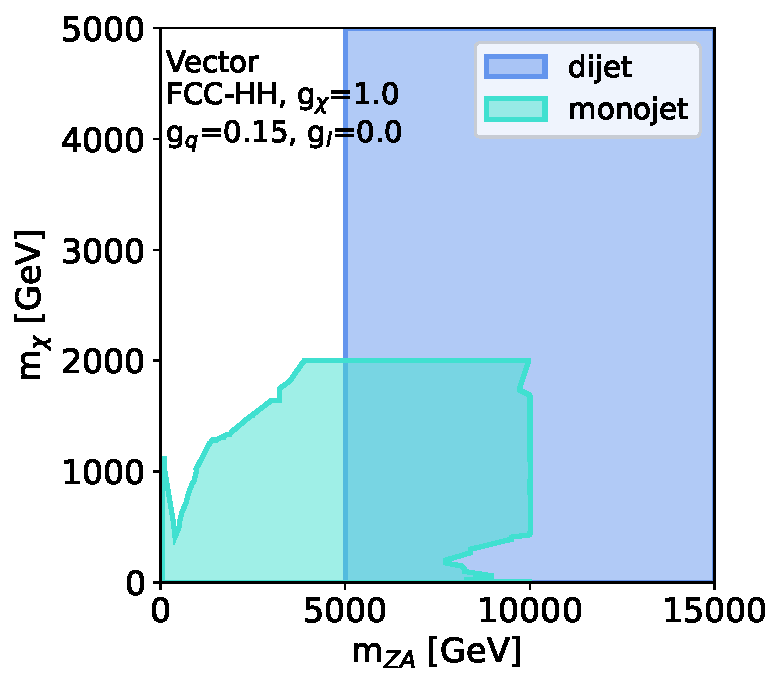
\includegraphics[width=\textwidth]{SummaryPlots-EF10/figures/massmass/fcc-hh/massmass_vector_gq0.15_gdm1.0_gl0.0.pdf}
         \caption{$g_q=0.15$, $g_{\chi}=1.0$, $g_l=0.0$}
         \label{subfig:vector-fcc-v1}
     \end{subfigure}
     \hfill
     \begin{subfigure}[b]{0.49\textwidth}
         \centering
         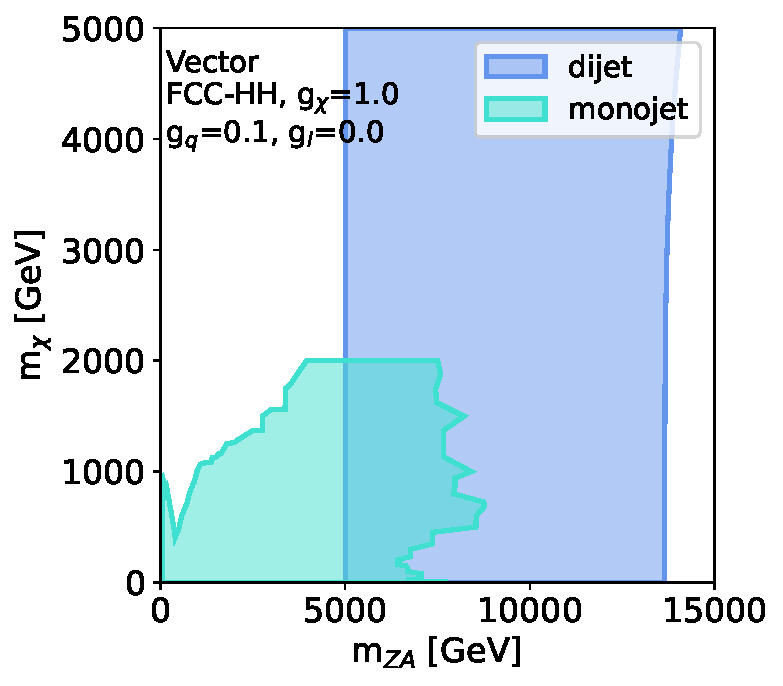
\includegraphics[width=\textwidth]{SummaryPlots-EF10/figures/massmass/fcc-hh/massmass_vector_gq0.1_gdm1.0_gl0.0.pdf}
         \caption{$g_q=0.1$, $g_{\chi}=1.0$, $g_l=0.0$}
         \label{subfig:vector-fcc-v2}
     \end{subfigure}

     \begin{subfigure}[b]{0.49\textwidth}
         \centering
         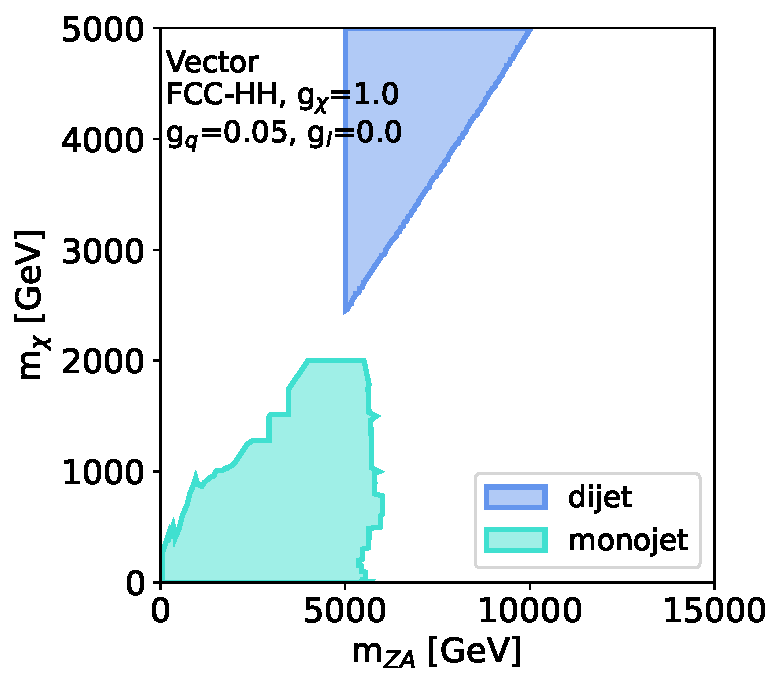
\includegraphics[width=\textwidth]{SummaryPlots-EF10/figures/massmass/fcc-hh/massmass_vector_gq0.05_gdm1.0_gl0.0.pdf}
         \caption{$g_q=0.05$, $g_{\chi}=1.0$, $g_l=0.0$}
         \label{subfig:vector-fcc-v3}
     \end{subfigure}
     \hfill
     \begin{subfigure}[b]{0.49\textwidth}
         \centering
         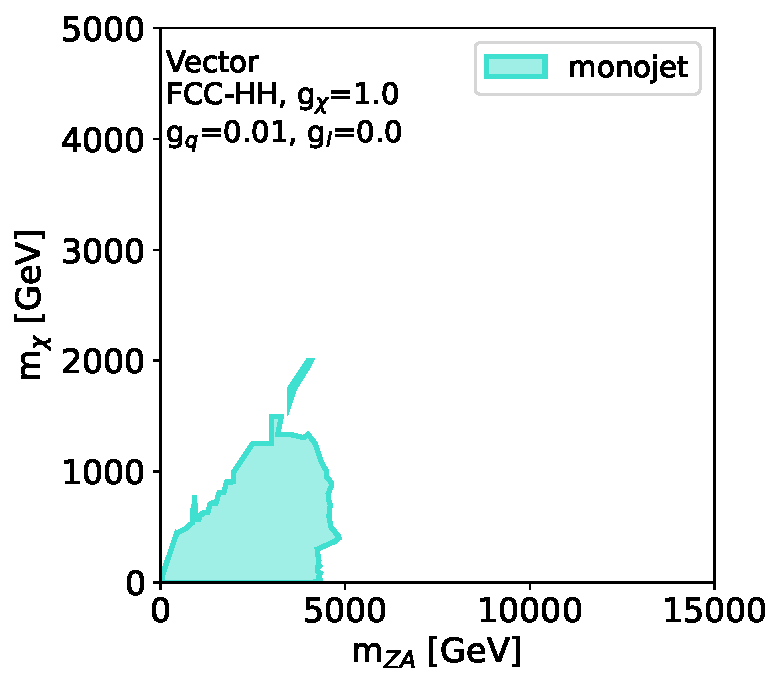
\includegraphics[width=\textwidth]{SummaryPlots-EF10/figures/massmass/fcc-hh/massmass_vector_gq0.01_gdm1.0_gl0.0.pdf}
         \caption{$g_q=0.01$, $g_{\chi}=1.0$, $g_l=0.0$}
         \label{subfig:vector-fcc-v4}       
     \end{subfigure}
        \caption{FCC-hh projected limits for individual analyses in the vector model and with a range of couplings. The truncation at the top of the monojet exclusion in subfigures~\ref{subfig:vector-fcc-v1,subfig:vector-fcc-v2} is due to a limitation in the input exclusion grid rather than a physical effect of the analysis at FCC-hh.}
        \label{fig:fcc-hh-massmass-separate}
\end{figure}

In Figure~\ref{fig:fcc-hh-massmass-combined}, combined exclusion contours are drawn for the FCC-hh monojet and dijet limits. In the absence of an effect from varying $g_l$, only one plane is illustrative and shows varied $g_q$. This is illustrated for both vector and axial-vector models.

\begin{figure}
     \centering
     \begin{subfigure}[b]{0.49\textwidth}
         \centering
         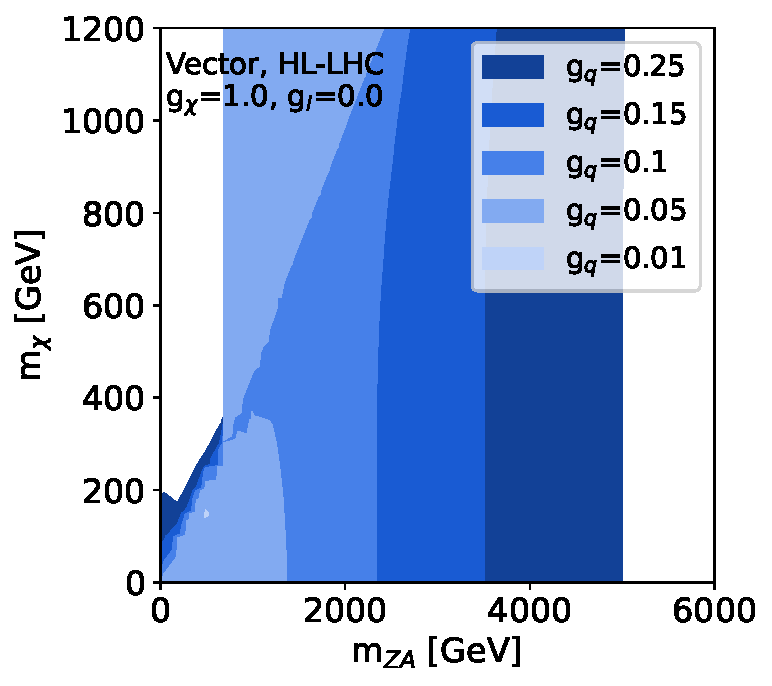
\includegraphics[width=\textwidth]{SummaryPlots-EF10/figures/massmass/hl-lhc/massmass_vector_gl0.0_gdm1.0.pdf}
         \caption{Effects on a vector model of varying $g_q$ coupling with no coupling to leptons}
         \label{subfig:vector-fcc-gqvariations1}
     \end{subfigure}
     \hfill
     \begin{subfigure}[b]{0.49\textwidth}
         \centering
         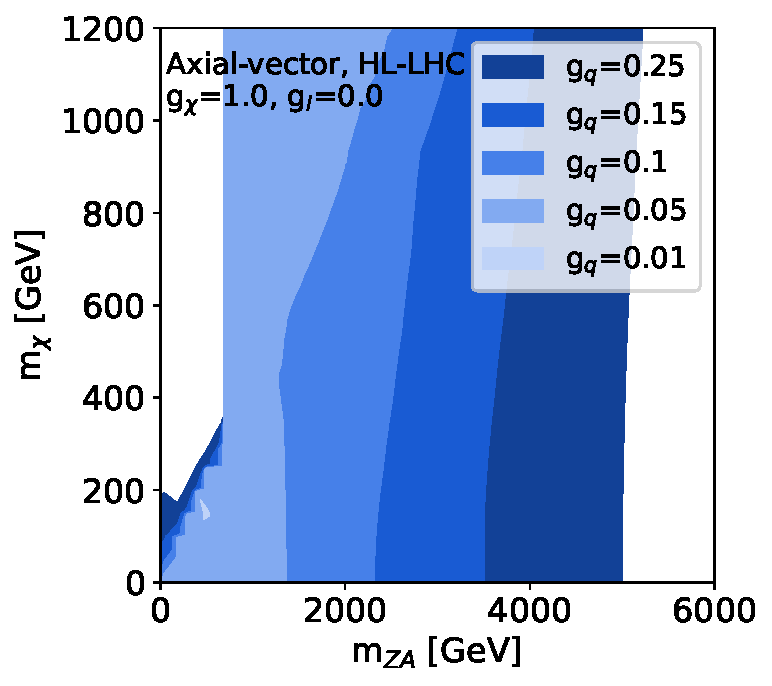
\includegraphics[width=\textwidth]{SummaryPlots-EF10/figures/massmass/hl-lhc/massmass_axial_gl0.0_gdm1.0.pdf}
         \caption{Effects on an axial-vector model of varying $g_q$ coupling with no coupling to leptons}
         \label{subfig:axial-fcc-gqvariations}
     \end{subfigure}
    \caption{FCC-hh projected limits, combined across analyses, for varying coupling values.}
    \label{fig:fcc-hh-massmass-combined}
\end{figure}

{\color{red}KP's next task: gq plots}

\section{Comparisons to other experiments}

\subsection{Previous text from LOI}

To understand how present and future collider searches complement present and future ID and DD experiments, we also propose to compare collider searches together with other experiments using variables commonly employed by displaying indirect and direct detection results, using the methods recommended by the LHC Dark Matter Working Group (DM WG)~\cite{BOVEIA2020100365,ALBERT2019100377}. An example of such plots (using fixed mediator – quark couplings) is shown in Figure \ref{Fig:Fig2}~\cite{Ellis:2691414}. Here, we propose to use results from work undergoing in synergy between the LHC DM WG and the Snowmass community~\cite{LOIVaryingCouplings} on collider limits with lower mediator - quark coupling values, rather than only for the fixed coupling values proposed by the LHC DM WG ~\cite{BOVEIA2020100365,ALBERT2019100377} and used in the European Strategy Briefing Book~\cite{Ellis:2691414}. This work will allow us to have a more complete picture of the complementarity of collider DM searches with direct and indirect detection, as well as compare collider results with collaborations that are sensitive to much lower couplings, such as accelerator-based and fixed target experiments. 

We are particularly interested in how to improve these plots in cooperation with the DD, ID and astrophysics probes communities within the Cosmic Frontier (CF1, CF3) and to contribute to summary plots where DM collider results and projections are shown together with those of accelerator-based experiments within the Rare and Precision Frontier (RF6). 

% KP removing old figures.
%\begin{figure}[ht]
%\begin{tabular}{ll}
%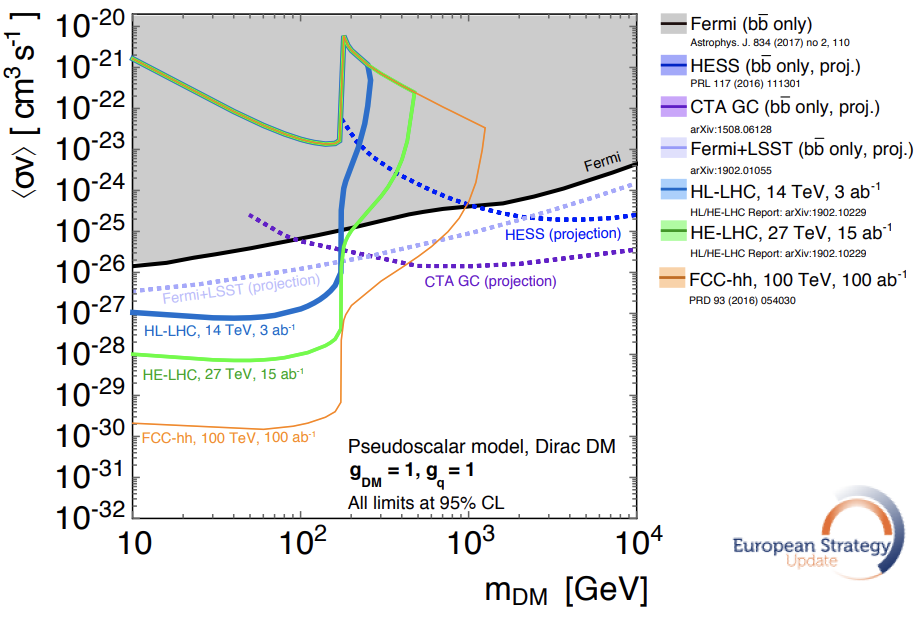
\includegraphics[scale=0.52]{figures/DMsummaryplots_ID.png}
%&
%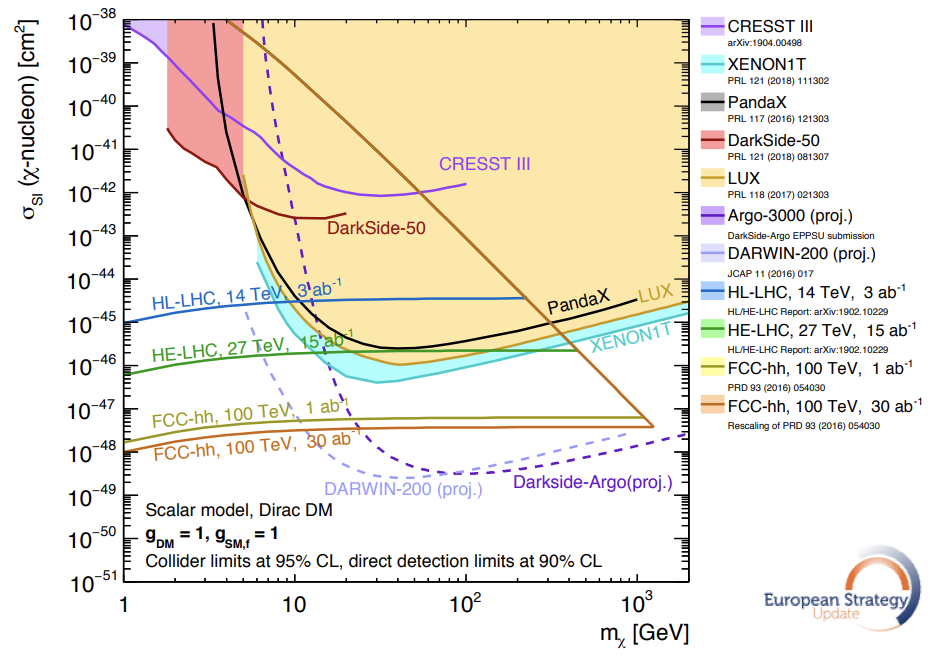
\includegraphics[scale=0.49]{figures/DMsummaryplots_DD.png}
%\end{tabular}
%\caption{{\bf Left panel}: comparison of projected limits from future %colliders with constraints from current and future ID experiments in the context of pseudo-scalar simplified model. All limits are shown at 95$\%$ CL. {\bf Right panel}: comparison of projected limits from future colliders with constraints from current and future DD experiments on the spin-independent DM–nucleon scattering cross section in the context of scalar simplified model. Collider limits are shown at 95$\%$ CL and direct detection limits at 90$\%$ CL. All panels adapted from~\cite{Ellis:2691414}.
%}
%\label{Fig:Fig2}
%\end{figure}

\subsection{Models considered}

Note something here? Here we should have dark photon and that DM model from Wisconsin in addition to the ones from the first section

\subsection{Results}

The exclusion limits for HL-LHC and FCC-hh in the vector and axial-vector models shown in the previous section have been converted into limits on the DM-nucleon interaction cross section. They are displayed for a similar range of couplings and are compared to existing direct detection limits in Figures~\ref{fig:hl-lhc-dd-separate-sd} and~\ref{fig:hl-lhc-dd-separate-si}.

\begin{figure}
     \centering
     \begin{subfigure}[b]{0.8\textwidth}
         \centering
         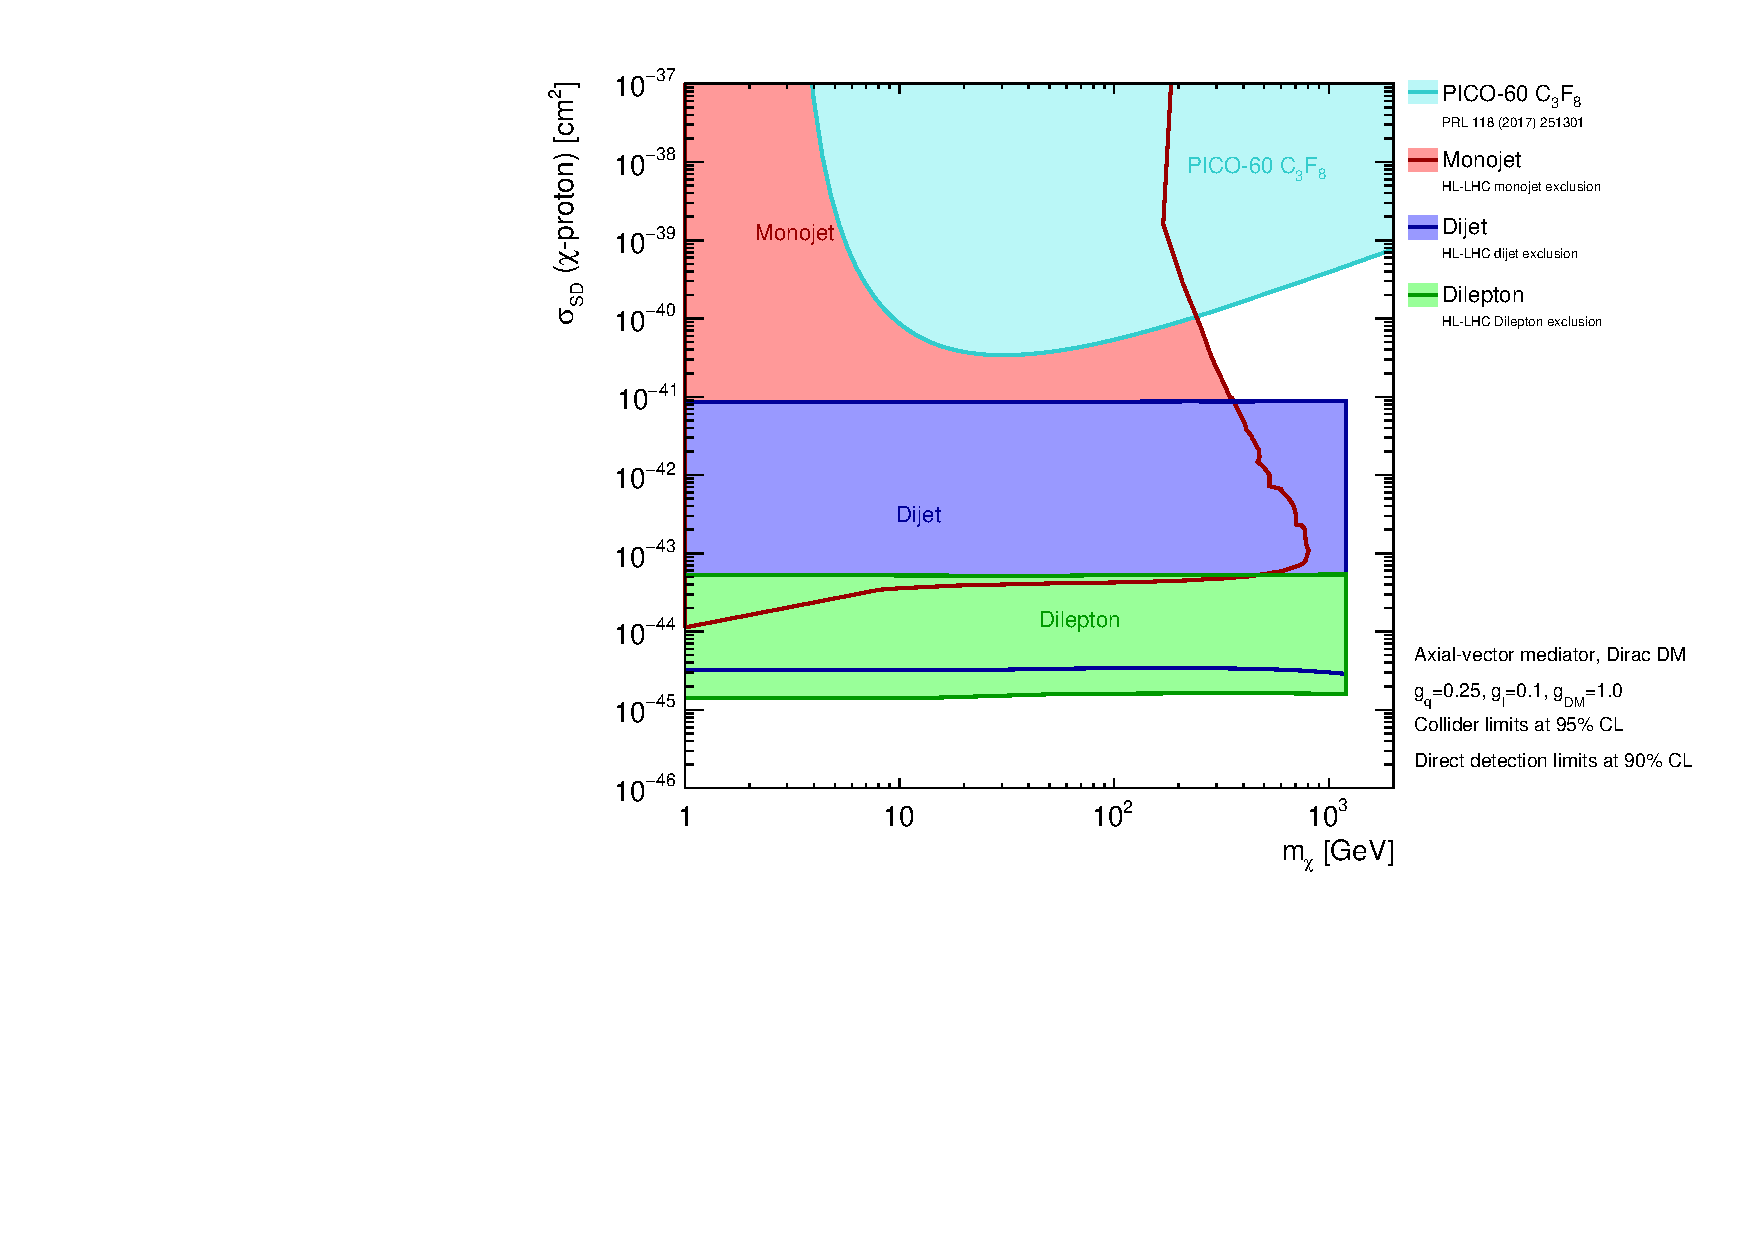
\includegraphics[width=\textwidth]{SummaryPlots-EF10/figures/directdetection/hl-lhc/DD_Axial-vector_contour_monojet_gq0p25_gdm1p0_gl0p1_proton.pdf}
         \caption{$g_q=0.25$, $g_{\chi}=1.0$, $g_l=0.1$}
         \label{subfig:dd-hl-lhc-a1}
     \end{subfigure}

     \begin{subfigure}[b]{0.8\textwidth}
         \centering
         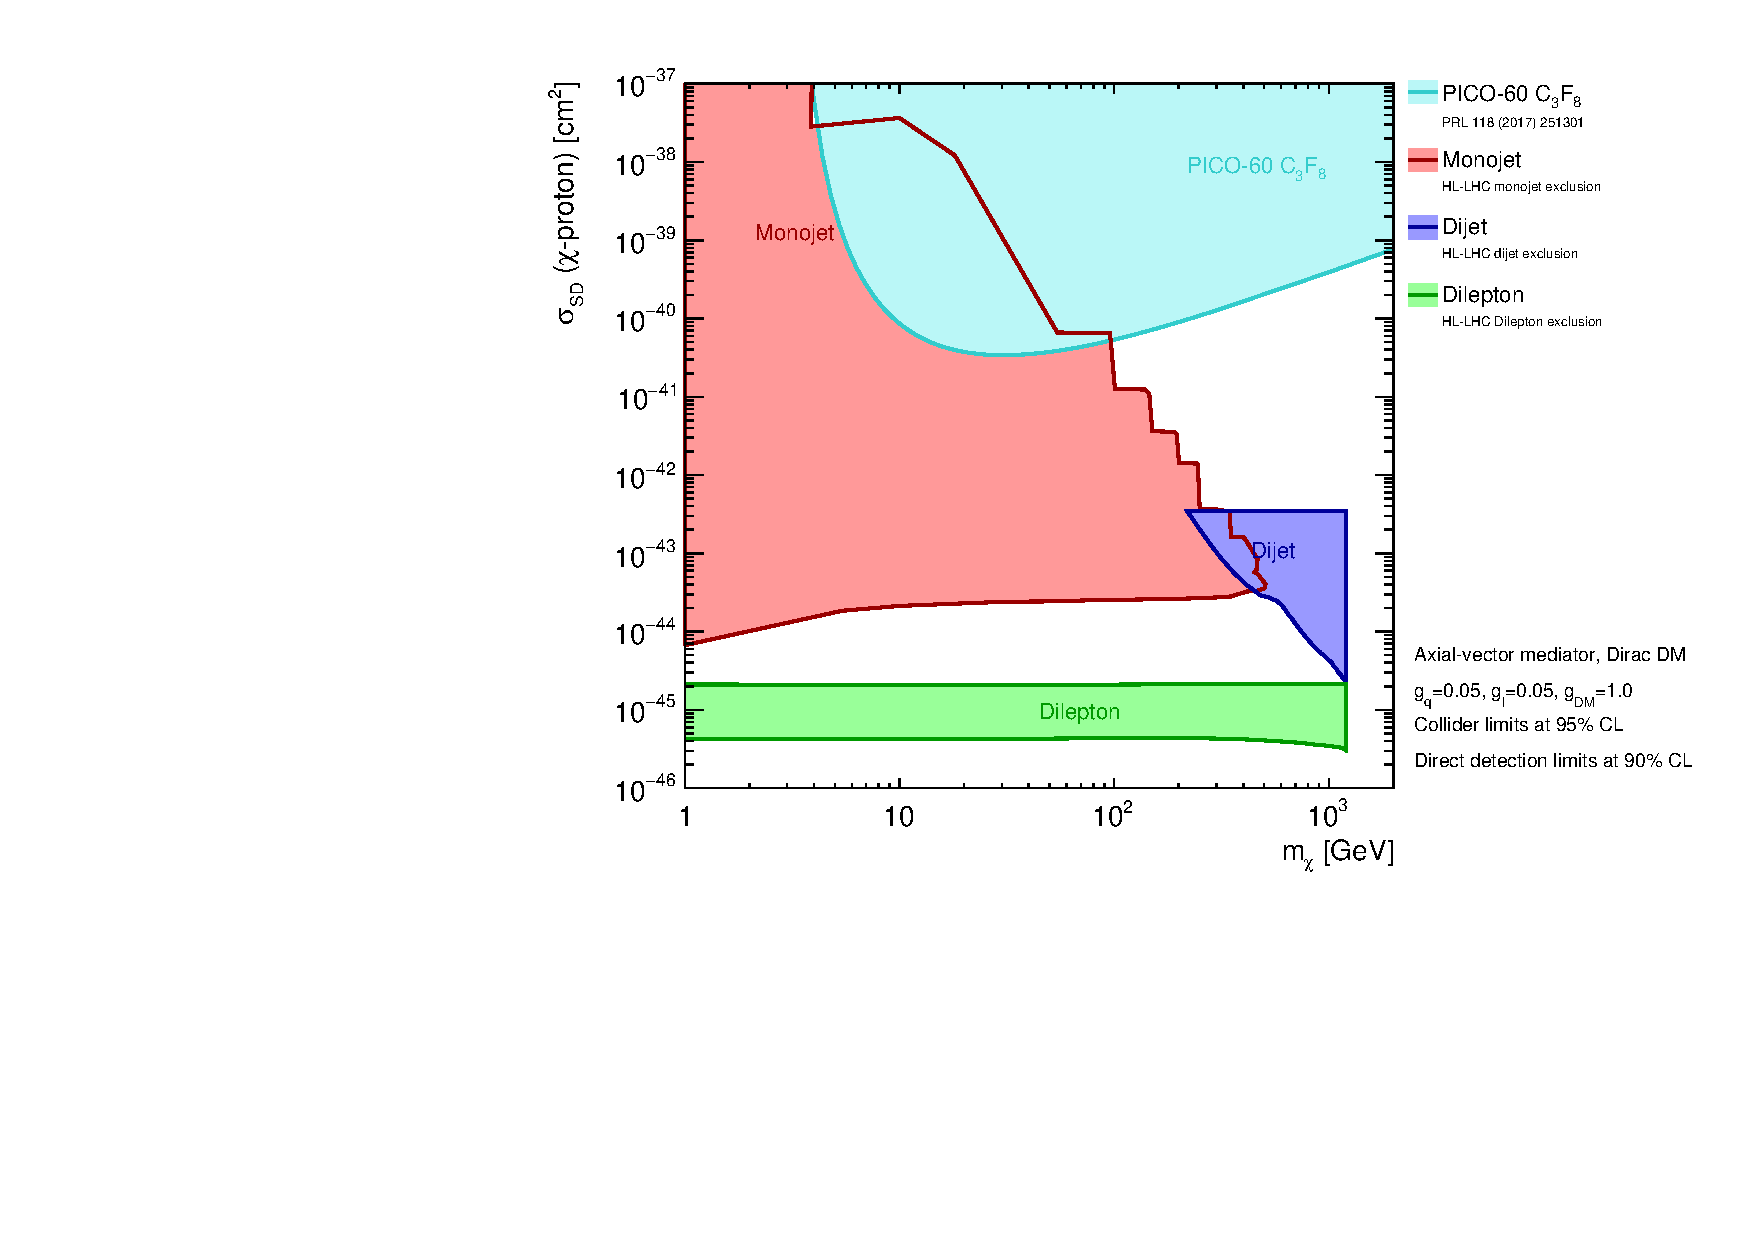
\includegraphics[width=\textwidth]{SummaryPlots-EF10/figures/directdetection/hl-lhc/DD_Axial-vector_contour_monojet_gq0p05_gdm1p0_gl0p05_proton.pdf}
         \caption{$g_q=0.05$, $g_{\chi}=1.0$, $g_l=0.05$}
         \label{subfig:dd-hl-lhc-new}
     \end{subfigure}
        \caption{Comparison of projected limits from HL-LHC with constraints from current DD experiments on the spin-dependent DM–proton scattering cross section in the context of the vector simplified model.}
        \label{fig:hl-lhc-dd-separate-sd}     
\end{figure}
     
\begin{figure}
     \centering
     \begin{subfigure}[b]{0.8\textwidth}
         \centering
         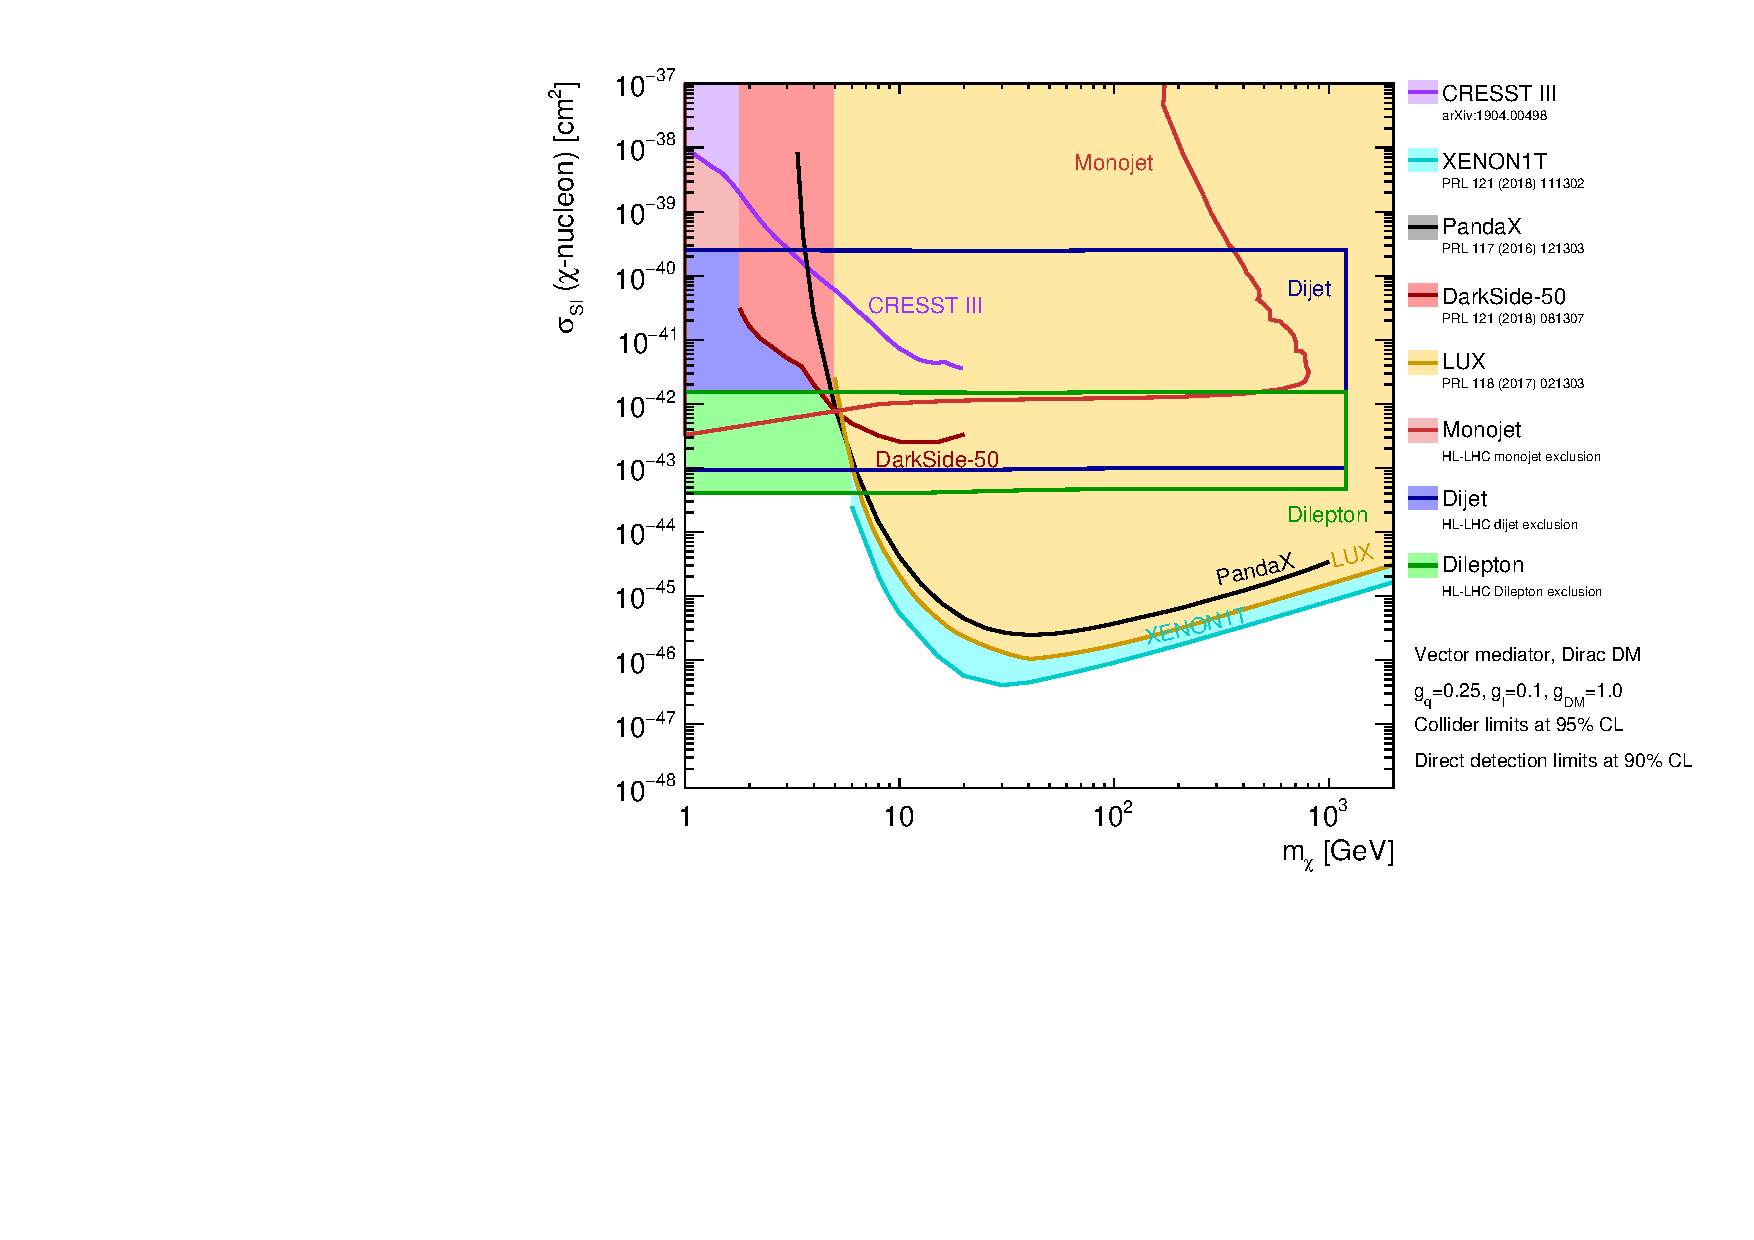
\includegraphics[width=\textwidth]{SummaryPlots-EF10/figures/directdetection/hl-lhc/DD_Vector_contour_monojet_gq0p25_gdm1p0_gl0p1_nucleon.pdf}
         \caption{}
         \label{subfig:dd-hl-lhc-a1}
     \end{subfigure}
     
     \begin{subfigure}[b]{0.8\textwidth}
         \centering
         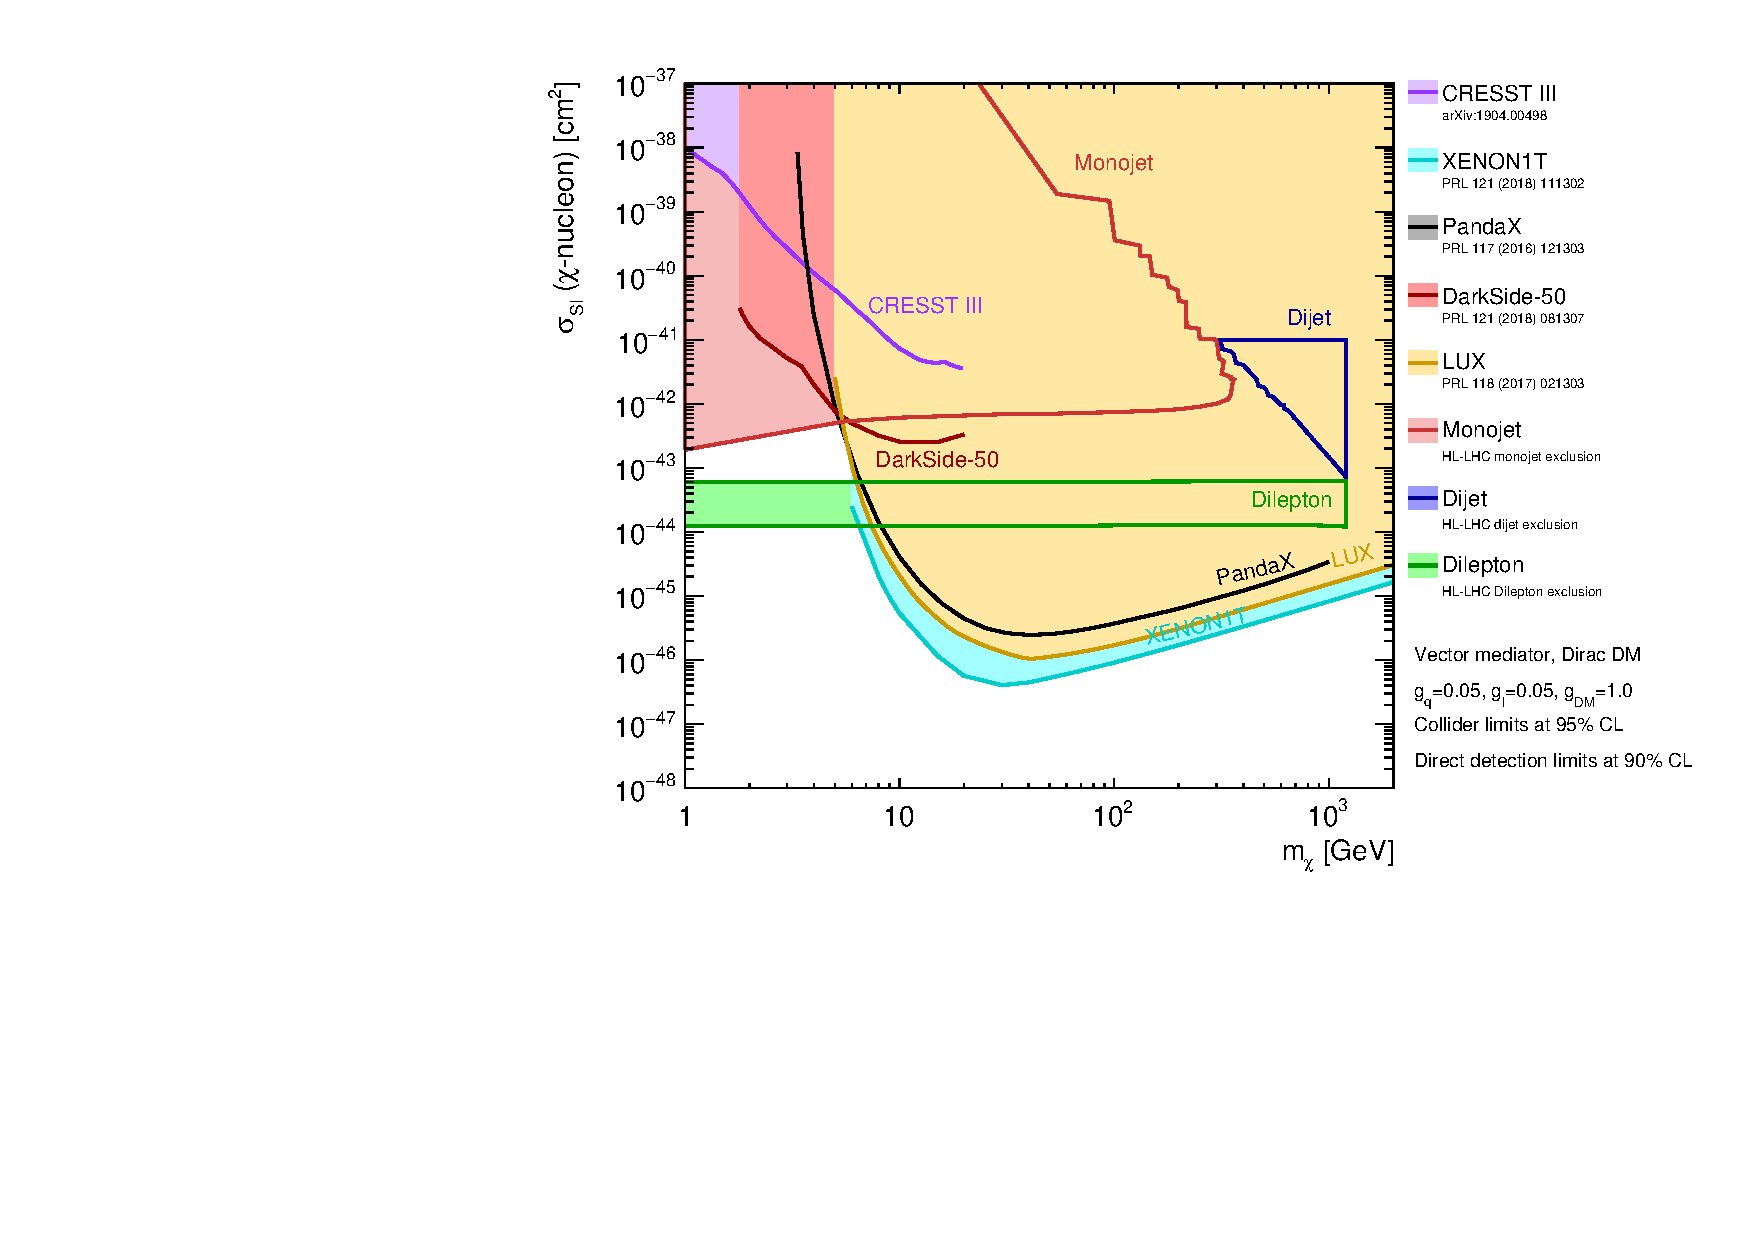
\includegraphics[width=\textwidth]{SummaryPlots-EF10/figures/directdetection/hl-lhc/DD_Vector_contour_monojet_gq0p05_gdm1p0_gl0p05_nucleon.pdf}
         \caption{}
         \label{subfig:dd-hl-lhc-vec}       
     \end{subfigure}
        \caption{Comparison of projected limits from HL-LHC with constraints from current DD experiments on the spin-independent DM–nucleon scattering cross section in the context of the vector simplified model.}
        \label{fig:hl-lhc-dd-separate-si}
\end{figure}

{\color{red}Here: add statement about how we will get projections for future experiments from cosmic frontier for final version}

{\color{red}Here: add KP's plots showing effects on DD limits of changing coupling, to illustrate degree of coupling independence of monojet exclusions}

\section{Reframing collider results as dark photon limits}

Phil, Josh: put dark photon plots here?
Include explanation of how equivalent the two models are and what settings are used to get these limits

\section{Dark matter projections for muon collider}

Deborah: put your plots here, with an explanation of the model used and how it's different from the one elsewhere in this paper?


\clearpage


%%%%%%%%%%%%%%%%%%%%%%%%%%%%%%%%%%%%%%%%%%

%  If you would like to use BibTEX for the bibliography, please feel free to do so.  It is not required.

%  To use BibTeX,

%    1.  uncomment the following two lines, 
%    2.  comment out everything below from  \begin{thebibliography}{99}   to \end{thebibliography).
%    3.  create the file  myreferences.bib, and process this file in the usual way

%\bibliographystyle{JHEP}
%\bibliography{myreferences}  % file myreferences.bib

%%%%%%%%%%%%%%%%%%%%%%%%%%%%%%%%%%%%%%%%%

\bibliography{Refs}


\end{document}



